% Version 01

\documentclass[a4paper]{article}
\pagestyle{empty}
\usepackage{amssymb}
\usepackage{amsmath}
\usepackage[dvips]{graphicx}
\setlength{\topmargin}{0.25in}
\setlength\headheight{0.25in}


\usepackage{fancyhdr,lastpage}
\pagestyle{fancy}
\chead{A Hybrid CFD/MD Simulation on Multi-physical Fluid System using SAGA and BigJob, Page \thepage~of 3}

%%% remove comment delimiter ('%') and specify parameters if required
%\usepackage[dvips]{graphics}

\begin{document}
\begin{center}

%%% remove comment delimiter ('%') and select language if required
%\selectlanguage{spanish} 

%%%%% TITLE %%%%%
\textbf {\bf \large A Hybrid CFD/MD Simulation on Multi-physical Fluid System 
using SAGA and BigJob}
\vspace{12pt}

%%%%% AUTHORS %%%%%
\textbf {Shantenu Jha$^1$, Nayong Kim$^1$, Soon-Heum Ko$^1$, Abhinav Thota$^1$, Joohyun Kim$^1$ and Dimitris Nikitopoulos$^2$}

\vspace{12pt}

%%%%% AFFILIATIONS %%%%%
\normalsize {$^1$ Center for Computation and Technology, \newline
Louisiana State University, Baton Rouge, LA 70803, USA}

\normalsize {$^2$Mechanical CityEngineering Department, \newline
Louisiana State University, Baton Rouge, LA 70803, USA}

\vspace{12pt}

\end{center}

%%%%% MAIN TEXT %%%%%
A hybrid CFD/MD approach [1,2] is a latest simulation method which adopts the continuum hypothesis in capturing the macroscopic features of a flowfield and resolves intermolecular effects on interfaces of different materials. CFD (Computational Fluid Dynamics) could accurately predict flow properties on conventional moderate/large size fluid domains, but is intrinsically impossible to reflect the characteristics of surrounding solid materials: MD (Molecular Dynamics) guarantees more accurate solution in that it also considers collision between fluid particles as well as interaction with solid particles, while its huge amount of computation time hinders from simulating a large scale system. Usually, continuum simulations are performed in fluid domains with bigger than hundreds of micrometers, while particle simulations are conducted nanometer levels. The need for simulating meso-scale systems in the middle of CFD and MD coverage and/or describing the effect of solid materials on fluid resulted in the development of a hybrid CFD/MD simulation model.

To conduct a tightly-coupled CFD/MD simulation, a hybrid scheme is implemented on reliable CFD and MD codes. An incompressible in-house code [3] based on artificial compressibility approach is employed to analyze the macroscopic features which are governed by the continuum equations. A famous LAMMPS package [4] is adopted for describing the particle dynamics near the solid material boundary where the interaction between the wall and the fluid takes place on the molecular level. Coupling schemes embedded on each code runs in the overlap region and data exchange takes place between CFD and MD domains.

The coupled simulation procedure is illustrated in Figure 1. At the start, CFD and MD codes solve their own governing equations, either mass and momentum conservation equations or placeCityNewton's second law. After two systems evolved the same physical time, they run their hybrid computation routine concurrently. This hybrid region minimally consists of five subzones. The CFD boundary zone is positioned in the bottom (i.e., nearest to the pure MD region). Velocities of particles within this zone are averaged and imposed as CFD boundary conditions for the corresponding computational cells. The MD boundary zone is placed above the CFD boundary zone. Here, velocities from the CFD grid are imposed on the MD through dynamically constrained MD equations. The dynamic constraint is introduced as a source term to the particle equation of motion which is appropriate to ensure that a macroscopic velocity from CFD and an averaged particle velocity from MD will eventually be the same. Between these zones, a buffer layer exists to transition the differences between the MD boundary and CFD boundary zones without direct influence of one on the other. On the top of the domain, an artificial force is applied to prevent particles from escaping from the hybrid region. A buffer layer is also placed between the constrained MD and the ``retaining'' force regions to prevent the artificial force field from influencing constrained MD solution directly.

Meanwhile, conducting this coupled simulation requires a lot of cautions. As CFD and MD codes have frequent communications, (e.g., the CFD code conducts data exchange in every iteration) they should start concurrently though they are totally separate packages. Users' account loss is inevitable in conventional queuing systems except when sufficient CPUs are idling, as the first running job has to wait its counterpart to follow. Even in cases with sufficient available resources, a user still experiences the unnecessary waste of his/her account for synchronized data exchange between two codes. Thus, a lot of manual endeavors are inevitable to do the load balancing between two jobs and to find a site with sufficient resource pool.

 Above hardships compelled to application scientists motivated us to use SAGA (the Simple API for Grid Applications) [5] and the BigJob abstraction [6]. SAGA represents (something by Shantenu) and the BigJob abstraction denotes (something by Shantenu). They let two application codes look like the unified one in the scheduler level and each job can be assigned with flexible number of processors within one BigJob.

The architecture of a BigJob and change of resource allocation to each task are schematized in Figure 2. The BigJob consists of computer scientific components such as SAGA CPR/Migol, SAGA Advert and a Replica-Agent, along with application softwares as their tasks. Also, the BigJob is closely connected with other middlewares such as Globus Toolkit [7] and schedulers. The simulation procedure became rather advanced for this tightly-coupled simulation, compared to former tests in which replica jobs were running independently with their own parameters and communicated at specified time for analysis and parameter change. When a BigJob is allocated, it starts running two application codes using predefined number of processors in each task. After a while, application codes conduct their own application-level checkpointing and they stop temporarily. Based on CPU usage until that time, BigJob reallocates processors to each task and application codes restart using their checkpointing data. When a new BigJob is added to the running simulation, the new one is merged onto the existing BigJob and simulation codes will restart with increased number of processors. This process is repeated until the simulation completes.

Three different tests are conducted to show the usefulness of the BigJob on tightly-coupled numerical simulations. To see the performance enhancement due to the dynamic execution, we have run one BigJob which contains CFD and MD tasks and checked the change of assigned number of processors with time. As a way of maximizing the use of available resources, we have submitted two BigJobs that conduct the identical coupled simulation and validated the merging of multiple BigJobs. Also, we have tested two BigJobs on heterogeneous systems to investigate the influence of multiple sites on the performance of BigJob.

\vspace{12pt}

%%%%% REFERENCES %%%%%
\parindent=0pt
{\bf References}
% \parindent=16pt
[1] REFERENCES HERE, p.~001-002, 2009.

\vspace{12pt}

%%%%% FIGURES %%%%%
% 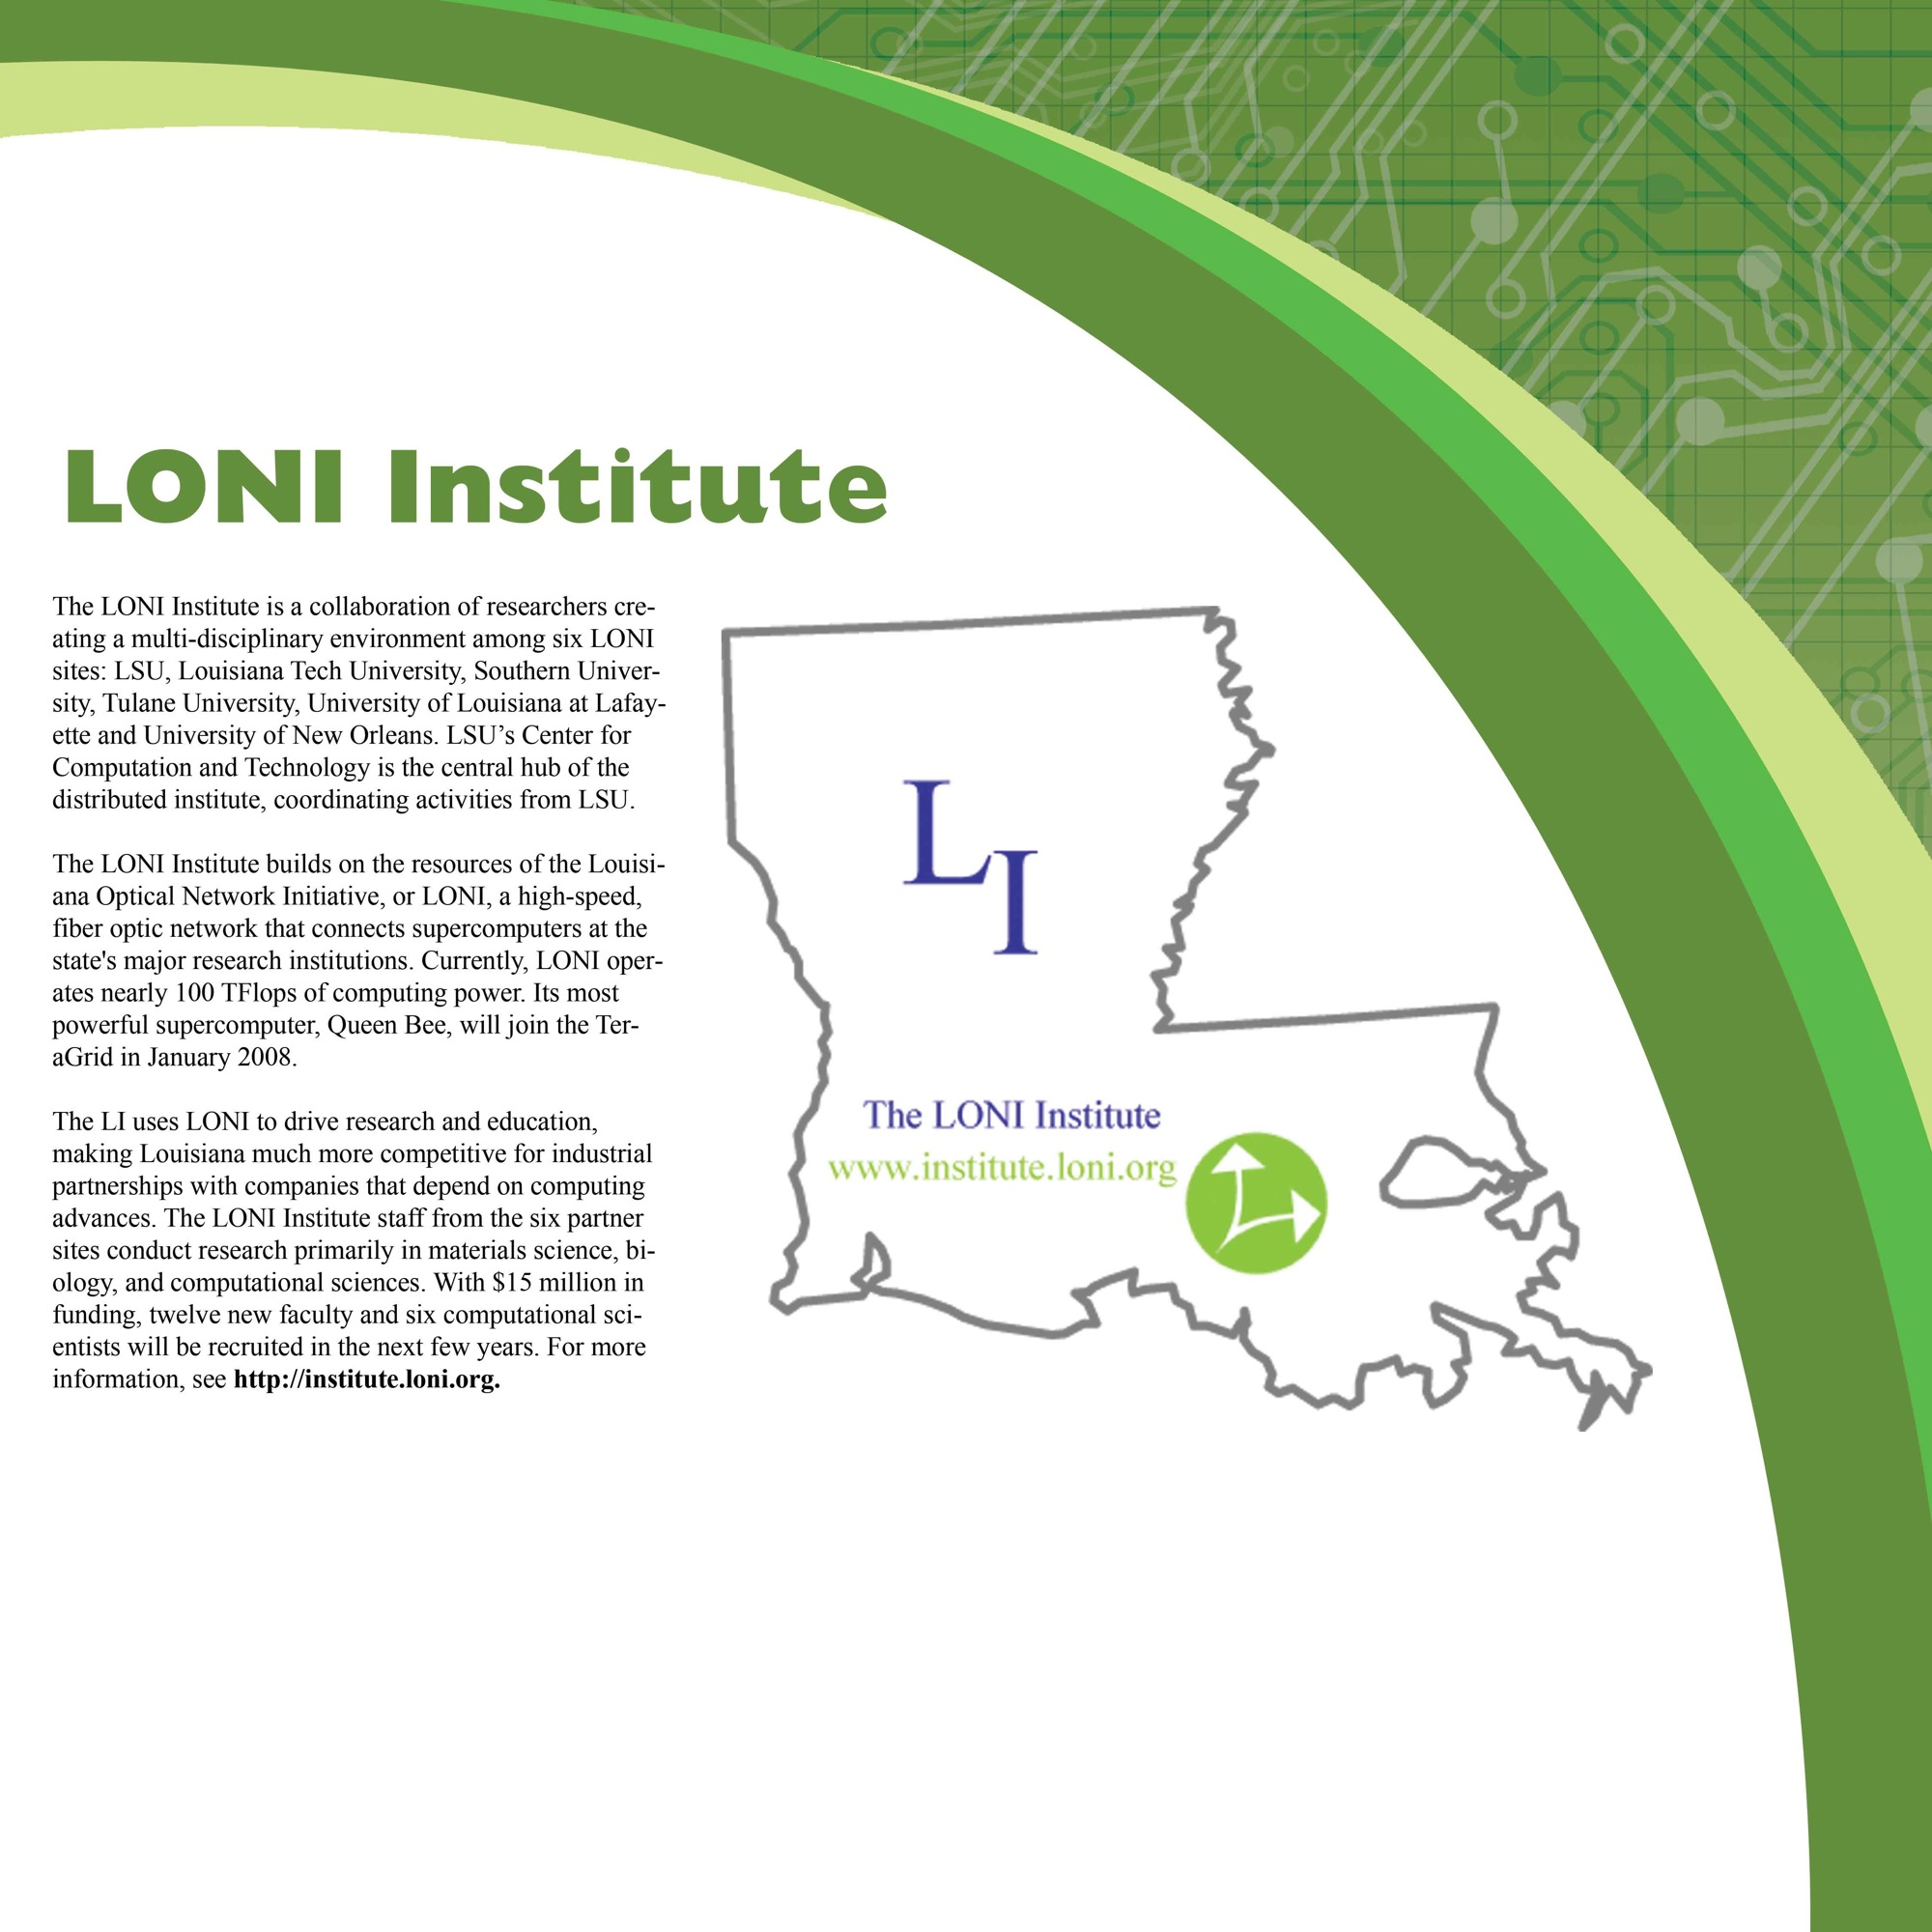
\includegraphics[bb=0mm 0mm 208mm 296mm, width=84.6mm, height=123.6mm, viewport=3mm 4mm 205mm 292mm]{image1.eps}
\begin{figure}
\centering
\includegraphics [scale=0.3]{fig1.eps}
\caption{Flowchart of CFD/MD Coupled Simulation}
%\label{sineplot}
%\textbf{Figure 1. Flowchart of CFD/MD Coupled Simulation}
\end{figure}

\begin{figure}
\centering
\includegraphics [scale=0.25]{fig2.eps}
\caption{Composition of a BigJob and Simulation Procedure}
%\label{sineplot}
%\textbf{Figure 1. Flowchart of CFD/MD Coupled Simulation}
\end{figure}


\noindent 

\end{document}


